\documentclass[11pt,a4paper]{article}
\usepackage[margin=2.4cm]{geometry}
\usepackage{amsmath,amssymb,booktabs,graphicx,hyperref,xcolor}
\usepackage[T1]{fontenc}
\graphicspath{{../figures/sigma0/}}
\hypersetup{colorlinks=true,linkcolor=blue!50!black,citecolor=blue!50!black,
            urlcolor=blue!50!black}
\newcommand{\Szero}{\ensuremath{\Sigma^{0}}}
\newcommand{\Lam}{\ensuremath{\Lambda}}
\newcommand{\uboone}{MicroBooNE}
\newcommand{\numubar}{\ensuremath{\bar{\nu}_\mu}}
\newcommand{\muUL}{\ensuremath{\mu_{\mathrm{UL}}}}
\emergencystretch=3em

\title{\Szero\ Production in the NuMI Beam at \uboone:\\ Analysis Note}
\author{J.~Nowak, N.~Patel}
\date{\today}

\begin{document}
\maketitle

\begin{abstract}
Working note for the \uboone\ search for \Szero\ production in $\numubar$
charged-current interactions in the NuMI beam, $\Szero\to\Lam\gamma$,
$\Lam\to p\pi^-$, with the full reverse-horn-current (RHC) exposure of
$1.15\times10^{21}$~POT. Two selections are maintained. The main one runs on
standard PeLEE ntuples, which carry data, beam-off (EXT) and dirt samples, and ends
in a cross-validated gradient BDT: $S=2.11$ NuWro signal events on $B=382$
($0.55\%$ purity). The second follows the \uboone\ \Lam\ CCQE analysis on
HyperonProduction ntuples, fitting the \Lam\ decay vertex and testing the
connectedness of the raw wire activity: $S=1.33$ GENIE signal events on $B=4.4$
($23\%$ purity), with no data or dirt in that format yet. An expected-sensitivity
calculation puts both under one signal model. Neither can observe \Szero\ at the
predicted rate, so the result will be an upper limit. The best median expected
90\%~CL limit is about $3\times$ the GENIE rate and $18\times$ the NuWro rate; the two
generators differ by a factor of six, because NuWro includes hyperon final-state
interactions. The PeLEE chain gives the better limit below a background
systematic of about $20\%$, and the two are within $10\%$ of each other up to $30\%$.
The background systematic of the PeLEE chain is therefore the next piece of work.
Revised 2026-10-19: the PeLEE background samples are complete (RHC dirt, the Run~3
overlay, EXT), the BDT is retrained with EXT, the \Lam-style chain and its EXT
estimate are documented, and the expected sensitivity is new
(Secs.~\ref{sec:samples}--\ref{sec:sensitivity}).
\end{abstract}

\tableofcontents

% =============================================================================
\section{Status and summary}
\label{sec:status}
% =============================================================================

The analysis sets a limit on \Szero\ production in $\numubar$ charged-current
interactions. The signature is
\begin{equation}
  \numubar + \mathrm{Ar} \to \mu^{+} + \Szero + X, \qquad
  \Szero \to \Lam\gamma, \qquad \Lam \to p\,\pi^{-},
\end{equation}
so the reconstructed final state is a muon, a proton, a pion and a photon of about
$75$~MeV. All yields in this note are scaled to the full RHC data exposure,
$1.1526\times10^{21}$~POT.

Two selections exist, on two ntuple formats, and they are fully independent
(Table~\ref{tab:chains}). The PeLEE chain (\texttt{Sigma/pelee/SigmaSelection.C},
Sec.~\ref{sec:pelee}) is the analysis: it is the only one that can see data, EXT and
dirt. The \Lam-style chain (\texttt{SigmaLambdaSel.C}, Sec.~\ref{sec:lambdastyle})
needs the raw wire activity, which only the HyperonProduction (``hypana'') format
stores, and that format exists for MC and EXT but not for data or dirt.

\begin{table}[h]\centering
\caption{The two selections at their operating points. GENIE yields use the
plain-overlay normalisation for both chains (Sec.~\ref{sec:rate}). Efficiencies are
quoted against each chain's own truth definition and are not comparable across
columns; the signal yields under one model are. $\muUL$ is the median expected 90\%~CL
limit on the rate in units of the model (Sec.~\ref{sec:sensitivity}).}
\label{tab:chains}
\small
\begin{tabular}{lll}
\toprule
 & PeLEE BDT & \Lam-style \\
\midrule
ntuple format & PeLEE & HyperonProduction \\
data, EXT, dirt & all three & EXT only (factorised) \\
final discriminant & BDTG $>0.759$ & island test on $\geq2$ planes \\
$S$, NuWro (with hyperon FSI) & $2.11$ & $0.142$ \\
$S$, GENIE (no hyperon FSI) & $13.1$ & $1.01$ \\
$B$ & $382$ & $4.40$ \\
purity, NuWro / GENIE & $0.55\%$ / $3.3\%$ & $3.1\%$ / $19\%$ \\
$\muUL$ at $f=15\%$, NuWro / GENIE & $48$ / $7.9$ (re-optimised $31$ / $5.0$) & $38$ / $5.4$ \\
\bottomrule
\end{tabular}
\end{table}

\paragraph{What changed since the previous version (2026-10-15).}
\begin{itemize}
  \item \textbf{PeLEE background samples completed} (Sec.~\ref{sec:samplechanges}).
        The dirt sample was FHC and is replaced by RHC dirt; the Run~3 overlay, $55\%$
        of the overlay statistics, was missing; the run3b beam-off (EXT) sample is
        added; and GENIE signal events inside the inclusive overlay are no longer
        counted as background.
  \item \textbf{BDT retrained} with EXT in the background tree and on $95\%$ of each
        cross-validation fold rather than the $50\%$ TMVA uses by default
        (Sec.~\ref{sec:bdt}). The figure of merit rises by $9.7\%$ and the background
        at the operating point halves.
  \item \textbf{Detector variations} measured on the PeLEE chain: $\lesssim7\%$ on
        the background, unresolved on the signal (Sec.~\ref{sec:detvar}).
  \item \textbf{The \Lam-style chain} is documented here for the first time
        (Sec.~\ref{sec:lambdastyle}). Its background now rests on $7.0\times10^{21}$~POT
        of hypana overlay, and the photon conversion gap is part of its operating point.
  \item \textbf{EXT for the \Lam-style chain}: a hypana EXT production and a
        factorised estimate, $0.62\pm0.27$ events (Sec.~\ref{sec:ext}).
  \item \textbf{Expected sensitivity} for both chains under one signal model
        (Sec.~\ref{sec:sensitivity}). This reverses the earlier conclusion, drawn
        from purity and from $S/\sqrt{S+B}$, that the \Lam-style chain is the
        stronger one.
\end{itemize}

\paragraph{What this analysis produces.} Not a differential cross section and not
an observation. The best median discovery significance at the predicted rate is
$0.6\sigma$ (GENIE) and $0.1\sigma$ (NuWro), so the deliverable is a cross-section
\emph{upper limit}. The PeLEE ntuples carry the multisim weights the background
covariance needs (\texttt{weightsGenie}, \texttt{weightsPPFX},
\texttt{weightsReint}), so this no longer depends on the framework port
(Sec.~\ref{sec:port}).

% =============================================================================
\section{Samples and normalisation}
\label{sec:samples}
% =============================================================================

\begin{table}[h]\centering
\caption{Samples, scaled to $1.1526\times10^{21}$~POT. The NuWro and dirt samples are
on the old NuMI flux and carry a per-event flux weight (mean $0.677$ for NuWro).}
\label{tab:samples}
\small
\begin{tabular}{llp{0.47\textwidth}r}
\toprule
format & sample & content & scale \\
\midrule
PeLEE & \Szero\ signal, other hyperons & NuWro run3b overlay, 249\,832 events, $1.3394\times10^{24}$~POT & $8.61\times10^{-4}$ \\
      & $\nu$ background & RHC overlay Runs 1, 2, 3, 4a, 4b, 4c, $1.5463\times10^{22}$~POT & $0.0745$ \\
      & dirt & RHC Runs 1, 2b, 3b, 4a, 4b, $1.7409\times10^{21}$~POT & $0.662$ \\
      & beam-off (EXT) & run3b, $3.265\times10^{7}$ gates & $0.750$ \\
\midrule
hypana & \Szero\ signal (GENIE) & \texttt{sig\_genie.list}, 4851 files, $5.9770\times10^{22}$~POT & $1.93\times10^{-2}$ \\
       & \Szero\ signal (NuWro) & the run3b production above & $8.61\times10^{-4}$ \\
       & $\nu$ background & \texttt{bkg\_overlay.list}, 14\,164 files, $7.0488\times10^{21}$~POT & $0.1635$ \\
       & beam-off (EXT) & 16\,570 events from 3\,349 run3b files, 162\,912 gates & $150.25$ \\
       & dirt, data & none & \\
\bottomrule
\end{tabular}
\end{table}

\subsection{The run3b NuWro signal production}

The Run~1-EXT sample \texttt{prod\_hyperon\_sigmazero\_reco1\_prodnuwro\_mcc9} was
retired on 2026-10-15. Its replacement is produced locally
(\texttt{\~{}/MicroBooNE/production/nuwro\_prod/}): 2500 jobs of 100 NuWro \Szero\
events overlaid on swizzled NuMI \textbf{run3b ext\_unbiased} data, through the full
gen$\to$reco2 chain, then both hypana and PeLEE ntuples.

\begin{center}
\begin{tabular}{lrr}
\toprule
 & retired (Run 1 EXT) & run3b \\
\midrule
files / events            & 2981 / 64716 & 2500 / 249832 \\
generated POT             & $3.4141\times10^{23}$ & $1.3394\times10^{24}$ \\
true \Szero\ CC $\numubar$ & 17714 ($27.4\%$) & 58545 ($23.5\%$) \\
raw signal at preselection & 3226 & 10931 \\
\bottomrule
\end{tabular}
\end{center}

\noindent The hypana \texttt{ana/MetaTree} sum and the merged PeLEE \texttt{SubRun}
sum agree on the POT to four digits, and \texttt{check\_ext\_unique.py} confirms
250{,}000 distinct EXT events with none used twice. The cosmics come from run3b, a
period the background overlay covers. Selection efficiency was unchanged by the swap
($50.1\% \to 50.8\%$ at preselection).

\subsection{The NuMI flux weight}

NuWro's flux files were converted from the \emph{old} NuMI gsimple flux (g4numi~v6,
bugged beamline geometry), while the overlay and the data are on the current
\texttt{g4\_10\_4} flux. Every NuWro event therefore carries the official
\uboone\ ``New/Old'' ratio weight, binned in $(E_\nu, \theta_{\mathrm{beam}})$. The
mean weight is $0.6774$, and $0.6770$ for the \Szero\ CC subset, flat to $0.1\%$ even
though those events sit $0.13$~GeV higher in energy. The only cost is a wider spread
(rms $0.297$ against $0.226$): $49.9$k effective events of $58.5$k.
\texttt{SigmaSelection.C} computes the weight from \texttt{nu\_e} and
\texttt{true\_nu\_p*}; the hypana macros read a per-event table. The RHC dirt turned
out to be on the old flux too (Sec.~\ref{sec:samplechanges}) and takes the same map.

\subsection{Changes to the PeLEE background samples (2026-10-17)}
\label{sec:samplechanges}

\begin{itemize}
  \item \textbf{The dirt was FHC.} The file used as ``Run~1 dirt''
        ($4.21\times10^{20}$~POT) has the true-$E_\nu$ spectra of the FHC dirt
        samples ($\chi^2/\mathrm{ndf}\approx1$) and not of the RHC ones
        ($\chi^2/\mathrm{ndf}$ 90--660): $\langle E\rangle$ for $\nu_\mu$ is $1.60$~GeV
        against $2.15$ for RHC, and for $\numubar$ $2.28$ against $1.72$. It is replaced
        by the RHC dirt of Runs 1, 2b, 3b, 4a and 4b ($1.7409\times10^{21}$~POT).
  \item \textbf{The RHC dirt is on the old NuMI flux.} Its \texttt{ppfx\_cv} profile in
        true $E_\nu$ matches the old-flux overlay in every bin ($\numubar$
        $0.886$--$0.910$ from 0 to 5~GeV) and not the current-flux overlay
        ($0.904$--$1.012$), so it takes the NuWro flux map.
  \item \textbf{The Run~3 overlay was missing}: five files, $5.5185\times10^{21}$~POT,
        $+55\%$ background statistics.
  \item \textbf{EXT added.} Run3b beam-off, $3.265\times10^{7}$ gates, scaled by
        $2.4477\times10^{7}$ beam-on triggers (the trigger table's $23\,534\,937$ per
        $1.10823\times10^{21}$~POT, taken at $1.1526\times10^{21}$): $0.7497$. Data
        files have \emph{empty} \texttt{backtracked\_*} vectors whenever there are
        PFPs, and the guard against ragged vectors had been dropping every
        neutrino-slice EXT event; it no longer requires them for data. The $1\,655$
        repeated (run, subrun, event) in the file are dropped.
  \item \textbf{Overlay signal removed from the background.} The inclusive overlay
        contains $1\,038$ raw GENIE \Szero\ signal events in the true fiducial volume,
        and they had been counted in $B$ while the NuWro sample models the signal. They
        are now kept out of $B$ and counted separately as the GENIE signal prediction
        (Sec.~\ref{sec:geniesig}).
\end{itemize}

\subsection{Why the samples disagree on the absolute \Szero\ rate}
\label{sec:rate}

On one truth definition and one fiducial volume, \Szero\ CC $\numubar$ events per
$1.1526\times10^{21}$~POT with the true vertex in the FV:

\begin{center}
\begin{tabular}{lrr}
\toprule
sample & in-FV \Szero\ & vs the plain overlay \\
\midrule
plain RHC overlay (unfiltered GENIE)      &  83.3 & 1.00 \\
GENIE hyperon sample \texttt{sig\_genie}  & 110.1 & 1.32 \\
NuWro run3b, POT scale only               &  18.9 & 0.23 \\
NuWro run3b, with the flux weight         &  12.8 & \textbf{0.15} \\
\bottomrule
\end{tabular}
\end{center}

\noindent The fiducial fractions are $37$--$38\%$ in all three, so this is not a
generation-volume artefact.

\paragraph{It is hyperon FSI.} The NuWro configuration
(\texttt{ultrapure-sigma0-numi-rhc.txt}) sets \texttt{dyn\_hyp\_cc=1} with every
other channel off and, within it, \texttt{hyp\_lambda=0},
\texttt{hyp\_sigma\_zero=1}, \texttt{hyp\_sigma\_minus=0}: NuWro generated the
\Szero\ channel \emph{and nothing else}, so its quoted POT per event is the exposure
per \Szero\ \emph{produced}. Everything else in the sample is final-state
interaction: of the $\numubar$ CC events only $25.3\%$ still carry a \Szero, $27.9\%$
carry a \Lam\ ($\Szero N \to \Lam N$ in the cascade), $10\%$ a $\Sigma^{\pm}$, and
$37.3\%$ no strange particle at all. The \uboone\ \Lam\ paper (arXiv:2212.07888)
states the other half outright: ``the NuWro predictions include the effect of final
state interactions, while GENIE does not take them into account''. For GENIE,
produced $=$ surviving, so the comparison that means anything is \Szero\
\emph{produced}:

\begin{center}
\begin{tabular}{lr}
\toprule
 & in-FV \Szero\ produced per full-RHC POT \\
\midrule
GENIE overlay (no hyperon FSI)      & 83.3 \\
NuWro, POT scale only               & 79.1 \\
NuWro, with the flux weight         & 53.6 \\
\bottomrule
\end{tabular}
\end{center}

\noindent The $6.5\times$ gap decomposes exactly as $4.19\times$ (FSI) $\times\,
1.48\times$ (flux weight) $\times\, 1.05\times$ (production rate), product
$6.51\times$ against the measured $6.51\times$. The sign flip between channels is
the same effect: in Fig.~2 of the \Lam\ paper NuWro sits \emph{above} GENIE
($\simeq2.1$ against $\simeq1.5 \times 10^{-40}$~cm$^2$/Ar) because FSI \emph{adds}
\Lam, and far below for \Szero\ because it \emph{removes} \Szero.

\paragraph{A control run verifies the normalisation.} The same flux, target and
configuration with \texttt{dyn\_hyp\_cc=0 dyn\_qel\_cc=1} -- ordinary CC
quasi-elastic instead of the hyperon channel -- gives $7.539\times10^{15}$~POT per
event over NuWro's box. The overlay's own CC QEL rate ($20{,}277$ in-FV events in
$7.1479\times10^{20}$~POT) converts to $8.835\times10^{15}$ on the same footing,
using the $37.0\%$ box-mass fiducial fraction and the $0.677$ flux factor. NuWro's
generic event rate is therefore within $17\%$ of GENIE's, the ordinary CCQE model
difference, and its flux $\times$ target normalisation is sound. Referenced to each
generator's own CCQE rate, NuWro's \Szero\ \emph{production} is $0.81\times$ GENIE's.

\paragraph{What this means for the limit.} A \Szero\ yield taken from the NuWro
sample is a yield \emph{with} hyperon FSI; one taken from the GENIE samples is a
yield \emph{without} it. The difference is roughly a factor of four and it is a model
choice, not a bug. The measured \Lam\ cross section,
$2.0^{+2.2}_{-1.7}\times10^{-40}$~cm$^2$/Ar, brackets both generators and cannot
distinguish them. Every result in this note is therefore quoted under both models.
The residual $1.3$--$1.6\times$ among the GENIE samples themselves -- the hyperon
sample's $1.32\times$ above, and the $1.61\times$ the \Lam\ cross-check of
Sec.~\ref{sec:lambdastyle} finds against the published GENIE prediction -- is
unexplained and separate. Where the two chains are compared under GENIE, both use
the plain-overlay normalisation.

% =============================================================================
\section{The PeLEE selection}
\label{sec:pelee}
% =============================================================================

\subsection{Signal definition and fiducial volume}
$\texttt{nu\_pdg} = -14$, $\texttt{ccnc} = 0$, a \Szero\ (PDG 3212) in the
final-state list \texttt{mc\_pdg}, a true muon momentum above $0.15$~GeV/$c$, no
other meson at the primary vertex, and the true vertex inside the fiducial volume.
The PeLEE truth record stops at the primary vertex, so the decay is tagged by the
\Szero\ itself, and no proton, pion or photon threshold can be imposed. The NuWro
PeLEE file has no \texttt{mc\_px}, so the muon threshold is \emph{not applied} to
the NuWro signal; it removes $4.2\%$ of signal muons where it can be applied. The
meson veto removes nothing from the NuWro sample.

Fiducial volume: $3.00 < x < 253.35$, $-112.53 < y < 114.47$, $3.1 < z < 1033.0$~cm,
excluding $675.1 < z < 775.1$~cm. This is looser than the CC$1\mu1\pi$ box: the
signal is rare enough that acceptance is worth more than vertex quality.

\subsection{Candidates and cut chain}
\begin{itemize}
  \item \textbf{Muon}: longest track with $\texttt{trk\_score}>0.8$, start within
        $20$~cm of the vertex, length $>10$~cm, LLR PID $>0.7$.
  \item \textbf{Proton and pion}: each non-muon track is scored for both roles with a
        quadratic logistic model and the best ordered pair is taken
        (\texttt{PidAssign.h}). Against HyperonProduction truth this raises the
        pion-candidate purity from $33.5\%$ (ranking on a single discriminant) to
        $42.5\%$; the ceiling is $51.4\%$, the fraction of selected signal that
        contains a reconstructed true $\pi^-$ at all. The candidates are formed when
        the tracks exist but are \emph{not required}: demanding them removed more signal
        than background ($-31.6\%/-18.3\%$ and $-52.9\%/-43.5\%$) and halved the figure
        of merit. Events without a pair carry sentinels and the BDT input
        \texttt{HasPair}.
  \item \textbf{Photon}: the non-track PFPs closest to the vertex; the closest is the
        \Szero\ decay photon. Its energy, from the per-PFP \texttt{shr\_energy\_y\_v},
        averages $70$~MeV in signal against the expected $74.5$~MeV.
\end{itemize}
Nine cumulative stages: \texttt{AllEvents}, \texttt{FiducialV},
\texttt{CosmicVeto} ($\texttt{topological\_score}>0.20$), \texttt{NShowers}
($0<n_{\mathrm{shr}}<4$), \texttt{MuonCandidate}, \texttt{ProtonCandidate} and
\texttt{PionCandidate} (pass-through, see above), \texttt{NTracksCut}
($n_{\mathrm{trk}}<5$), \texttt{BDTG}. Derived observables: \Lam\ and \Szero\
masses, \Lam\ and photon vertex-pointing angles and impact parameters, \Lam\ decay
distance, a $\pi^0$ di-photon mass, and the second-shower block of
Sec.~\ref{sec:glee}.

\subsection{BDT}
\label{sec:bdt}
Gradient BDT over 57 inputs, evaluated with two-fold cross-validation: folds are
trained on even and odd event numbers and each is applied only to the events it did
not train on. Every BDT number in this note is out of sample.

\paragraph{Retrained 2026-10-18.} Two changes, measured separately on the same
events with EXT in $B$:
\begin{enumerate}
  \item \textbf{EXT in the background tree.} The run3b beam-off events (8\,977 raw,
        $25\%$ of the training background weight) were not in the previous training.
  \item \textbf{Train on $95\%$ of each fold.} TMVA's default splits each fold into
        train and test halves; the test half feeds only TMVA's overtraining printout,
        so each fold trained on $25\%$ of all events.
\end{enumerate}

\begin{center}
\resizebox{\textwidth}{!}{%
\begin{tabular}{lcccccc}
\toprule
training & AUC & \multicolumn{3}{c}{$B/B_0$ at signal efficiency} & \multicolumn{2}{c}{peak $S/\sqrt{S+B}$} \\
 & & $50\%$ & $40\%$ & $20\%$ & value & cut \\
\midrule
2026-10-15 (no EXT, half fold)       & 0.8894 & 0.0412 & 0.0253 & 0.0067 & 0.0993 & 0.690 \\
EXT, half fold (3 seeds)             & 0.8956--0.8966 & 0.0378--0.0385 & 0.0228--0.0236 & 0.0059--0.0062 & 0.1037--0.1049 & \\
\textbf{EXT, 95\% of fold (adopted)} & \textbf{0.9000} & \textbf{0.0358} & \textbf{0.0215} & \textbf{0.0061} & \textbf{0.1077} & \textbf{0.759} \\
EXT, 95\% of fold (2 other seeds)    & 0.9002--0.9017 & 0.0352--0.0354 & 0.0209--0.0213 & 0.0059--0.0060 & 0.1084--0.1092 & \\
\bottomrule
\end{tabular}}
\end{center}

\noindent EXT in the training gives $+5\%$ in the figure of merit, almost all of it
EXT rejection: at $50\%$ signal efficiency $0.9\%$ of the EXT survives against $2.2\%$,
with the overlay rate unchanged. Training on the full fold gives another $+4\%$, and
every full-fold seed beats every half-fold seed; reseeding moves the figure of merit
by only $\pm0.5\%$. That the BDT still improves when it sees more signal is the
signal-statistics limit again. The default seed is adopted, not the best one.

\subsection{Results}
\label{sec:peleeresults}

\begin{table}[h]\centering
\caption{PeLEE chain at the operating point $\mathrm{BDTG}>0.759$. Efficiency is raw
signal against true \Szero\ in the FV. $B$ = other hyperons $+$ overlay $+$ dirt $+$
EXT.}
\label{tab:perf}
\begin{tabular}{lrrrrrr}
\toprule
stage & raw signal & eff.\ [\%] & $S$ & $B$ & purity [\%] & $S/\sqrt{S+B}$ \\
\midrule
MuonCandidate & 11107 & 51.61 & 6.469 & 28978 & 0.022 & 0.0380 \\
NTracksCut    & 10931 & 50.79 & 6.370 & 26549 & 0.024 & 0.0391 \\
\textbf{BDTG} & \textbf{3644} & \textbf{16.93} & \textbf{2.110} & \textbf{382.4} & \textbf{0.549} & \textbf{0.1076} \\
\bottomrule
\end{tabular}
\end{table}

\begin{center}
\begin{tabular}{lrrr}
\toprule
$B$ at the BDTG point & previous BDT, cut 0.616 & current BDT, cut 0.759 & raw events \\
\midrule
other hyperons (NuWro) & 1.74 & 1.06 & 1841 \\
overlay                & 715.7 & 367.9 & 5178 \\
dirt                   & 13.8 & 2.26 & 7 \\
EXT                    & 109.5 & 11.25 & 15 \\
\midrule
total                  & 840.7 & 382.4 & \\
$S$                    & 2.850 & 2.110 & 3644 \\
\bottomrule
\end{tabular}
\end{center}

\noindent The previous column is the previous BDT with the completed samples, EXT
included. At MuonCandidate EXT is $6\,844$ events against $20\,348$ from the overlay;
after the BDT it is $3\%$ of the background. Figure~\ref{fig:bdt} shows the score.

\begin{figure}[h]\centering
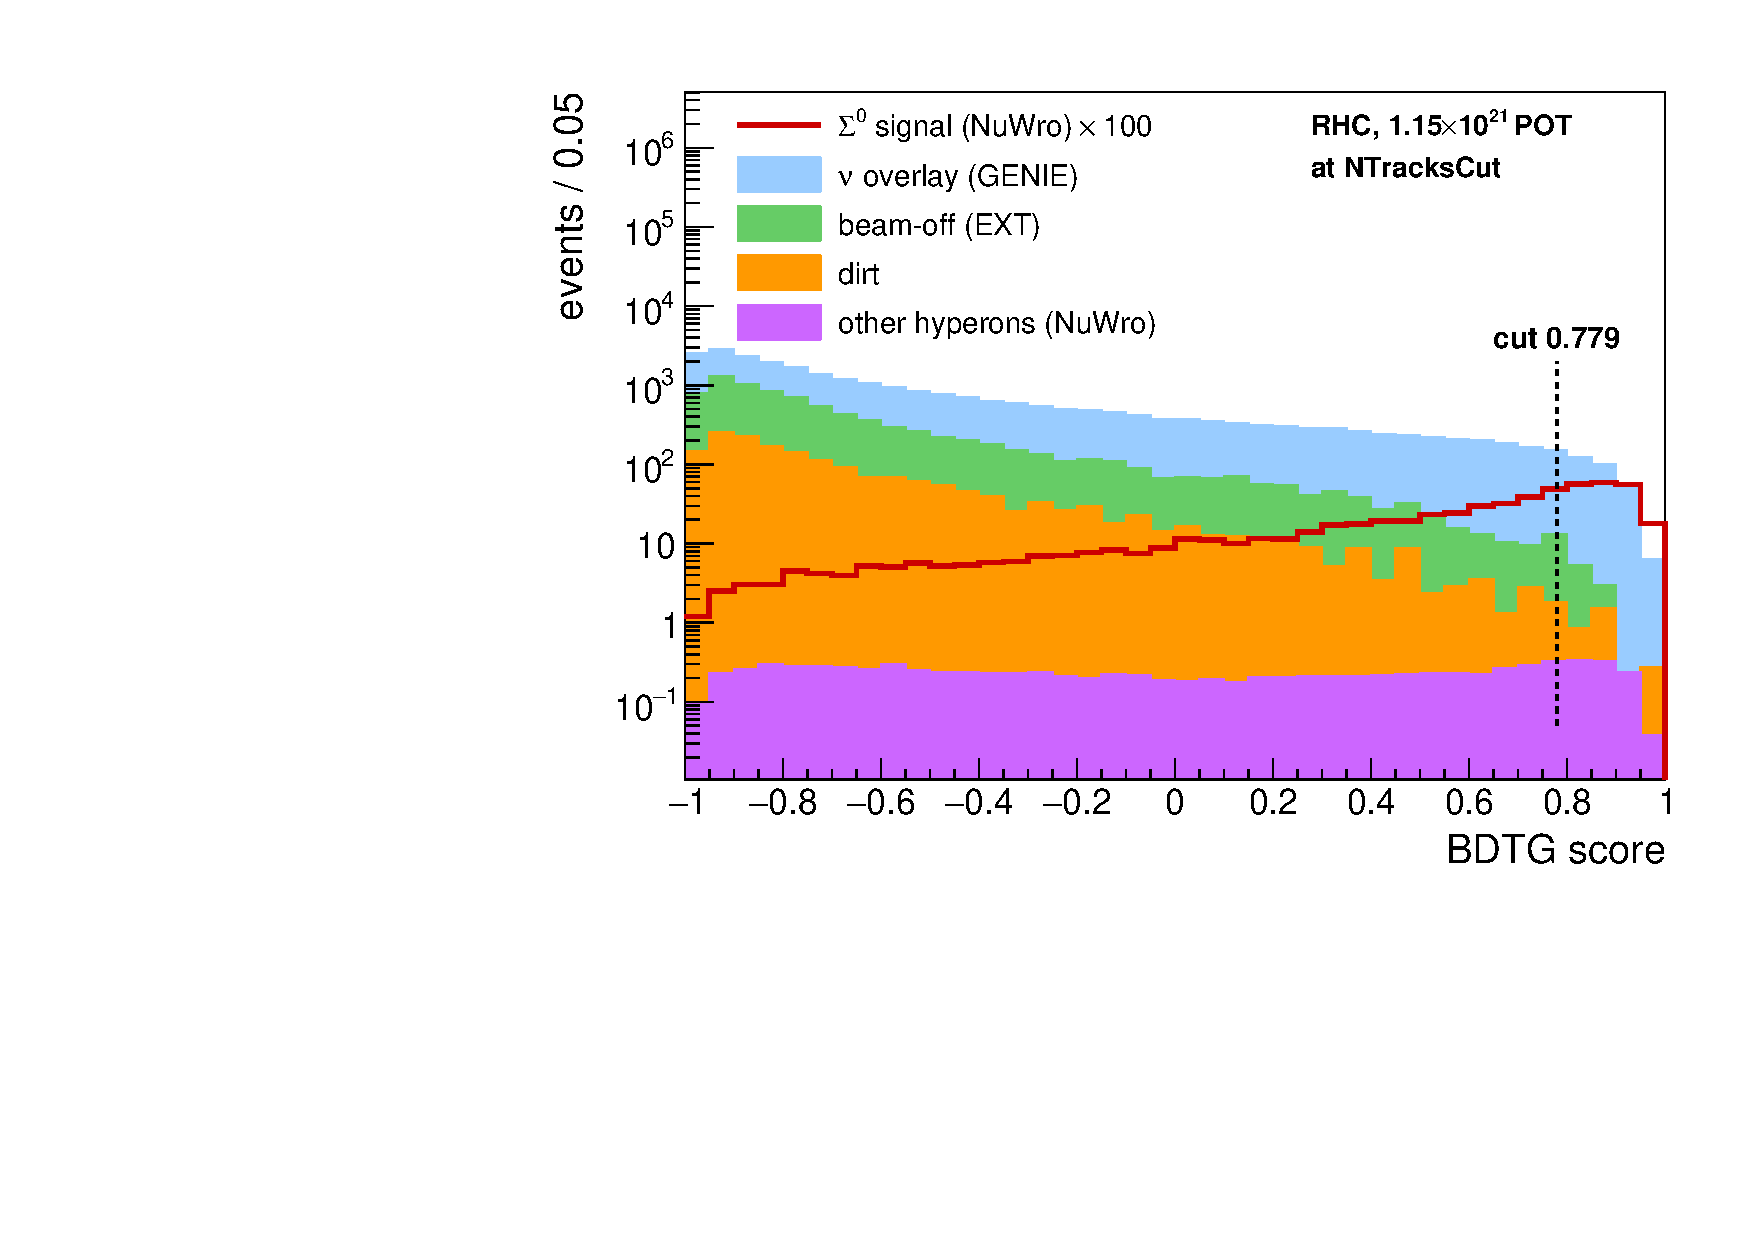
\includegraphics[width=0.7\textwidth]{bdt_score.pdf}
\caption{Cross-validated BDTG score at \texttt{NTracksCut}, background stacked by
sample and the NuWro signal scaled by 100. The dashed line is the operating point.}
\label{fig:bdt}
\end{figure}

\paragraph{The operating point should follow the systematic budget.} $0.759$ is the
peak of $S/\sqrt{S+B}$. There a $2\%$ background systematic is $\pm7.6$ events against
$2.1$ signal, and the figure of merit cannot see it. Section~\ref{sec:sensitivity}
chooses the cut by the expected limit instead: $0.750$ at $f=0$, $0.875$ at $10\%$,
$0.890$ at $15\%$.

\subsection{GENIE signal through the same selection}
\label{sec:geniesig}
The overlay's own GENIE \Szero\ events (Sec.~\ref{sec:samplechanges}) are run through
the full selection and BDT and counted apart from every sample, so the PeLEE chain
has a GENIE signal yield under the same definition. The BDT never trains on them.

\begin{center}
\begin{tabular}{lrrrr}
\toprule
stage & raw & $S_{\mathrm{GENIE}}$ & efficiency [\%] & GENIE/NuWro \\
\midrule
AllEvents (true FV)  & 1038 & 72.56 & 100   & 5.78 \\
MuonCandidate        &  553 & 38.67 & 53.3  & 5.98 \\
NTracksCut           &  544 & 38.08 & 52.5  & 5.98 \\
BDTG                 &  187 & $13.09\pm1.01$ & 18.0 & 6.20 \\
\bottomrule
\end{tabular}
\end{center}

\noindent The efficiencies agree: $18.0\%$ for GENIE against $16.8\%$ for NuWro
(weighted), a ratio of $1.07\pm0.08$. The limit on the number of signal events is
therefore model-independent to a few percent; what depends on the model is the rate
it is compared with.

\subsection{Detector variations}
\label{sec:detvar}
The Run~3 RHC detector-variation set re-simulates the same generated events under
nine variations. \texttt{run\_detvar.sh} runs the selection on each file and
\texttt{DetVar.C} compares each variation with the CV on the events they share, with
the CV weight on both sides. The samples are on the old flux, so only the ratios are
used.

\begin{center}
\begin{tabular}{lrr}
\toprule
variation & $S$ var/CV & $B$ var/CV \\
\midrule
LY attenuation   & $1.000\pm0.000$ & $0.997\pm0.005$ \\
LY down          & $0.975\pm0.025$ & $0.985\pm0.006$ \\
LY Rayleigh      & $0.980\pm0.039$ & $0.987\pm0.008$ \\
recombination    & $1.062\pm0.088$ & $0.973\pm0.030$ \\
SCE              & $0.921\pm0.090$ & $0.998\pm0.034$ \\
WireMod $\theta_{XZ}$ & $0.907\pm0.076$ & $1.002\pm0.023$ \\
WireMod $\theta_{YZ}$ & $0.840\pm0.078$ & $1.026\pm0.026$ \\
WireMod $X$      & $0.975\pm0.075$ & $1.027\pm0.026$ \\
WireMod $YZ$     & $0.964\pm0.095$ & $0.986\pm0.023$ \\
\midrule
quadrature (MC noise alone) & $21.7\%$ ($21.1\%$) & $5.2\%$ ($6.8\%$) \\
\bottomrule
\end{tabular}
\end{center}

\noindent No variation is resolved on either side: both quadrature sums equal their MC
noise. The CV keeps 51 raw signal and 1\,260 raw background events at this cut, so the
detector systematic is bounded at $\lesssim7\%$ on the background ($\pm27$ events) and is
not measured on the signal. WireMod $\theta_{YZ}$ ($2.0\sigma$) and $\theta_{XZ}$
($1.2\sigma$) pull the signal down, as they did at the previous operating point.

% =============================================================================
\section{What limits the PeLEE purity}
\label{sec:purity}
% =============================================================================

The studies in this section were made on earlier versions of the chain (before the
joint assignment, the 2026-10-18 retraining and the completed samples). The
fractions carry over; the absolute yields do not.

\paragraph{The surviving background is $\pi^0$ events.}
\begin{table}[h]\centering
\caption{Surviving background by interaction mode, at a looser earlier operating
point.}
\begin{tabular}{lrr}
\toprule
Mode & Scaled yield & \% of background \\
\midrule
Resonant (RES)       & 1381.8 & 52.3 \\
Deep inelastic (DIS) &  635.3 & 24.0 \\
Quasi-elastic (QE)   &  363.8 & 13.8 \\
Meson exchange (MEC) &  177.1 &  6.7 \\
Cosmic               &   74.6 &  2.8 \\
Coherent (COH)       &    8.9 &  0.3 \\
\midrule
Total                & 2643.1 & 100 \\
\bottomrule
\end{tabular}
\end{table}

\noindent RES and DIS together are $76\%$. Both produce $\pi^0 \to \gamma\gamma$,
which supplies a fake \Szero\ photon, plus charged hadrons that fake the proton and
pion tracks. The background is not diffuse: it is one physics process.

\paragraph{The candidate assignment is the weak link.} Truth-matched purities of the
candidates in background events, before the joint assignment: muon $81\%$, proton
$58\%$, pion $31\%$ (another proton $28\%$), photon $29\%$ (a proton $18\%$). The pion
and photon candidates are wrong roughly $70\%$ of the time, so both masses are built
from misidentified objects in most background events. Section~\ref{sec:recostudy}
measures the same on signal, on the hypana ntuples.

\subsection{The photon candidate}
\label{sec:photonstudy}

Truth-matching the photon candidate in background (69\,557 preselected events):
photon $30.0\%$, unmatched $26.7\%$, charged pion $16.3\%$, proton $15.2\%$, muon
$9.8\%$, electron $1.4\%$. Charged tracks reconstructed as showers are $41\%$.

\paragraph{The signal photon is soft, which inverts the strategy.} The
$\Szero$--$\Lam$ mass splitting is only $77$~MeV, so
\begin{equation}
  E_\gamma = \frac{m_{\Szero}^2 - m_{\Lam}^2}{2 m_{\Szero}} = 74.5~\mathrm{MeV}
\end{equation}
in the \Szero\ rest frame. The photon candidate averages $70$~MeV in signal and
$140$~MeV in background, where $\pi^0$ photons dominate. Requiring shower-like quality
would remove signal preferentially. Cuts in the soft direction help at preselection
($E_\gamma<120$~MeV: $94.5\%$ of signal, $25.4\%$ of background removed, figure of
merit $\times1.09$) but not on top of the BDT ($\times1.012$), which already uses the
photon energy. An explicit $\pi^0$ mass veto rejects only $9\%$ of background, because
it needs \emph{two} reconstructed showers. The shower Moli\`ere angle, the one unused
shape variable, was added to the BDT and changed the figure of merit by $\times1.013$.

\subsection{Methods taken from the single-photon analyses}
\label{sec:glee}

The gLEE single-photon search and the NC$\pi^0$ technote isolate a single photon
against $\pi^0$ events in which one decay photon was missed, which is our problem.
\begin{enumerate}
  \item \textbf{Second-Shower Veto variables} -- evidence of a photon that was not
        reconstructed: the unassociated-hit count and fraction in the slice
        (recomputed per event), \texttt{slclustfrac}, \texttt{secondshower\_Y\_nhit},
        \texttt{secondshower\_Y\_dot} and the sub-cluster counts. \emph{In the BDT}:
        they are among the 57 inputs.
  \item \textbf{One BDT per background class} ($\pi^0$, non-$\pi^0$ neutrino, cosmic)
        instead of one BDT for everything. \texttt{TrainBDTSplit.C},
        \texttt{apply\_split.C} and \texttt{eval\_split.C} implement it; it was run
        once on a 1\,004-signal-event tree and has not been compared with the
        current single BDT. A split of the training by \texttt{HasPair} was measured
        and does not help.
  \item \textbf{Conversion distance} as a first-class variable: realised in the
        \Lam-style chain as the photon gap (Sec.~\ref{sec:lambdastyle}).
  \item \textbf{Constrain the $\pi^0$ rate from data.} The NC$\pi^0$ technote finds
        GENIE over-predicts non-coherent NC$\pi^0$ by $25\%$. Our background is the
        same physics, so its normalisation belongs in the covariance and, with data,
        in a sideband constraint (Sec.~\ref{sec:plan}).
\end{enumerate}

% =============================================================================
\section{Reconstruction study on HyperonProduction ntuples}
\label{sec:recostudy}
% =============================================================================

\subsection{Why the PeLEE ntuples cannot answer these questions}

Every question about \emph{which particle a candidate actually is} is unanswerable
on the PeLEE ntuples: \texttt{mc\_pdg} lists the \Szero\ and the muon, but never the
$\Szero \to \Lam\gamma \to p\pi^-\gamma$ chain, and \emph{zero of 17721 signal events}
contain a backtracked $\pi^-$ PFP. The HyperonProduction analyser writes the full
decay chain together with per-PFP truth matching (\texttt{pfp\_true\_pdg},
\texttt{pfp\_purity}, \texttt{pfp\_completeness}). \texttt{HypInput.h} adapts the
hypana branches to the PeLEE names the selection uses.

Three things to know about the format. It has no implicit neutrino-slice
requirement: PeLEE events without a neutrino slice die at the fiducial cut, but
hypana attaches a vertex to them anyway, which inflated the background $2.4\times$
until the explicit \texttt{flash\_match\_nu\_slice\_ID}~$\geq0$ stage was added; the
two chains then agree to $6$--$8\%$ throughout. Its \texttt{trk\_energy\_proton} is
the proton \emph{momentum}, not the kinetic energy that the PeLEE branch of the same
name holds; with the conversion the \Lam\ mass width falls from $23.5$ to $7.8$~MeV
(half inter-quartile range), and the PeLEE chain was never affected. And its
\texttt{pfp\_true\_origin} is the analyser's own enum (2 is a \Lam\ daughter), not
\texttt{simb::Origin}. The measurements below were made on the retired NuWro
sample; they are efficiencies and ratios, which the swap does not move.

\subsection{Signal definition used in this section}

\Szero, $\numubar$ charged current, $\Lam \to p\pi^-$ in truth, muon momentum above
$0.15$~GeV/$c$, and \textbf{both} the reconstructed and the true vertex inside the
FV. Only $\sim 60\%$ of \Szero\ events have $\Lam \to p\pi^-$ at all (PDG $63.9\%$).
Requiring only the \emph{reconstructed} vertex in the FV gives badly wrong answers:
events whose reco vertex is in the FV but whose true vertex is not are
mis-reconstructed, and they dominate. With reco FV only, the muon appears to be
reconstructed $53.7\%$ of the time and all four particles $10.2\%$; with both, $91.5\%$
and $18.1\%$.

\subsection{Per-particle reconstruction}

\begin{table}[h]\centering
\begin{tabular}{lrrrr}
\toprule
particle & primary (gen 2) & secondary (gen $\geq3$) & not reconstructed & total \\
\midrule
$\mu^+$   & $91.5\%$ & $0.3\%$ & $8.2\%$  & $91.8\%$ \\
$p$       & $58.1\%$ & $2.8\%$ & $39.1\%$ & $60.9\%$ \\
$\pi^-$   & $45.7\%$ & $1.6\%$ & $52.8\%$ & $\mathbf{47.3\%}$ \\
$\gamma$  & $59.8\%$ & $2.6\%$ & $37.6\%$ & $62.4\%$ \\
\bottomrule
\end{tabular}
\caption{Reconstruction of the four \Szero\ final-state particles (3704 signal
events). The $\pi^-$ is the weak link.}
\label{tab:recoeff}
\end{table}

All four are found together in $18.1\%$ of events, the hard ceiling for any selection
that requires all four. Secondaries do not explain the loss: keeping generation-3
PFPs (new \texttt{pfp\_generation} branch) recovers only $2.8\%$ for the proton and
$1.6\%$ for the pion.

\subsection{Track/shower misclassification}

In events with at least four PFPs, with the selection's split
(\texttt{pfp\_trk\_shr\_score}~$>0.5$): the muon is a track $95.7\%$ of the time,
the proton $70.3\%$, the pion $54.2\%$ (a shower $11.6\%$), and the photon is a
\emph{track} $15.0\%$ of the time. All four are found in $41.2\%$ of these events but
correctly classified in only $26.7\%$. Photons passing as tracks compete for the pion
slot, which is the origin of the $25\%$ photon contamination among pion candidates.

\subsection{The pion candidate}

On signal reaching the pion stage, a true $\pi^-$ PFP exists in only $56.6\%$ of
events, and $76.3\%$ have exactly one track-like PFP left after the muon and proton
are taken. The joint assignment of \texttt{PidAssign.h} (Sec.~\ref{sec:pelee}) is the
improvement that was available; raising the pion track-score threshold lifts purity
but lowers the figure of merit monotonically.

\subsection{The \Lam\ flight distance from the primary vertex is not measurable}

Measured with truth-matched $p$ and $\pi^-$ tracks ($n=266$): the true \Lam\ flight
has median $1.85$~cm and mean $3.23$~cm ($\beta\gamma \approx 0.4$, so
$\beta\gamma c\tau \approx 3$~cm), the reconstructed primary-vertex resolution is
$5.54$~cm, and the reconstructed and true flight distances are uncorrelated
($r=-0.014$). Three decay-vertex estimators give the same $\sim5.5$~cm residual, all
limited by the primary vertex; the tracks themselves converge well (DCA median
$0.33$~cm).

\paragraph{What this does not rule out.} The measurement kills a cut on the distance
between the Pandora vertex and the decay point. It does not kill the displaced
topology: the \Lam-style chain (Sec.~\ref{sec:lambdastyle}) fits the decay vertex
from the two tracks, requires the pair momentum to point back at the event vertex,
and tests at wire level whether the pair is separated from the muon. That test passes
$80\%$ of signal with $2$--$3$~cm flight and $98.6\%$ of the signal it keeps has
flown more than $2$~cm.

% =============================================================================
\section{The \Lam-style selection}
\label{sec:lambdastyle}
% =============================================================================

\subsection{Motivation}

The \uboone\ \Lam\ CCQE analysis (Thorpe \& Nowak, Hyperon Technote v2) selects
$\numubar$ CC \Lam\ with $91\%$ purity. At the same $6.7\%$ efficiency the earlier
hypana BDT chain for \Szero\ had $2.8\%$. Three causes were identified: our
preselection rejected long-flight \Lam\ (the pion score penalised tracks displaced
from the primary vertex), there were no pair-level requirements, and the photon is
an extra object. Reimplemented on our files (\texttt{LambdaSel.C}), their chain
reproduces their efficiency to $0.79\times$ (our pair selector is provisional and
their decay BDT is replaced by cuts), but the GENIE signal normalisation comes out
$1.61\times$ theirs, which is unexplained and affects every \Szero\ yield.
\texttt{SigmaLambdaSel.C} follows their chain.

\subsection{What it does differently}
\begin{itemize}
  \item \textbf{Every ordered track pair is scored}, not each track separately. The
        pair selector's only topological input is the separation of the two track
        starts, which does not penalise a \Lam\ that flew.
  \item \textbf{Pair precuts are a preference, not a veto}: as a veto they cost
        $\sim20\%$ of signal at the same figure of merit.
  \item \textbf{The decay vertex is fitted} (a V fit, which recovers $3.78$~cm for a
        true $4.00$~cm flight), giving a decay length and the pointing angle $\alpha$
        between the pair momentum and the vertex-to-decay direction.
  \item \textbf{The island test is a cut}, applied last.
\end{itemize}

\subsection{The island test}

A wire $\times$ time grid of the stored activity is built on each plane, clusters
are seeded at the muon, proton and pion track starts, and the test requires the
proton and pion clusters to merge while the muon stays separate
(Fig.~\ref{fig:island}). The coordinate transforms were derived and validated for
this ($\mathrm{wire} = (Ay+Bz+C)/0.3$ reproduces $98.7\%$ of the stored vertex wires
within two wires; $\mathrm{tick} = 18.1509\,x + 818.1$). The test reads raw wire
windows, which exist only in the hypana format.

\begin{figure}[h]\centering
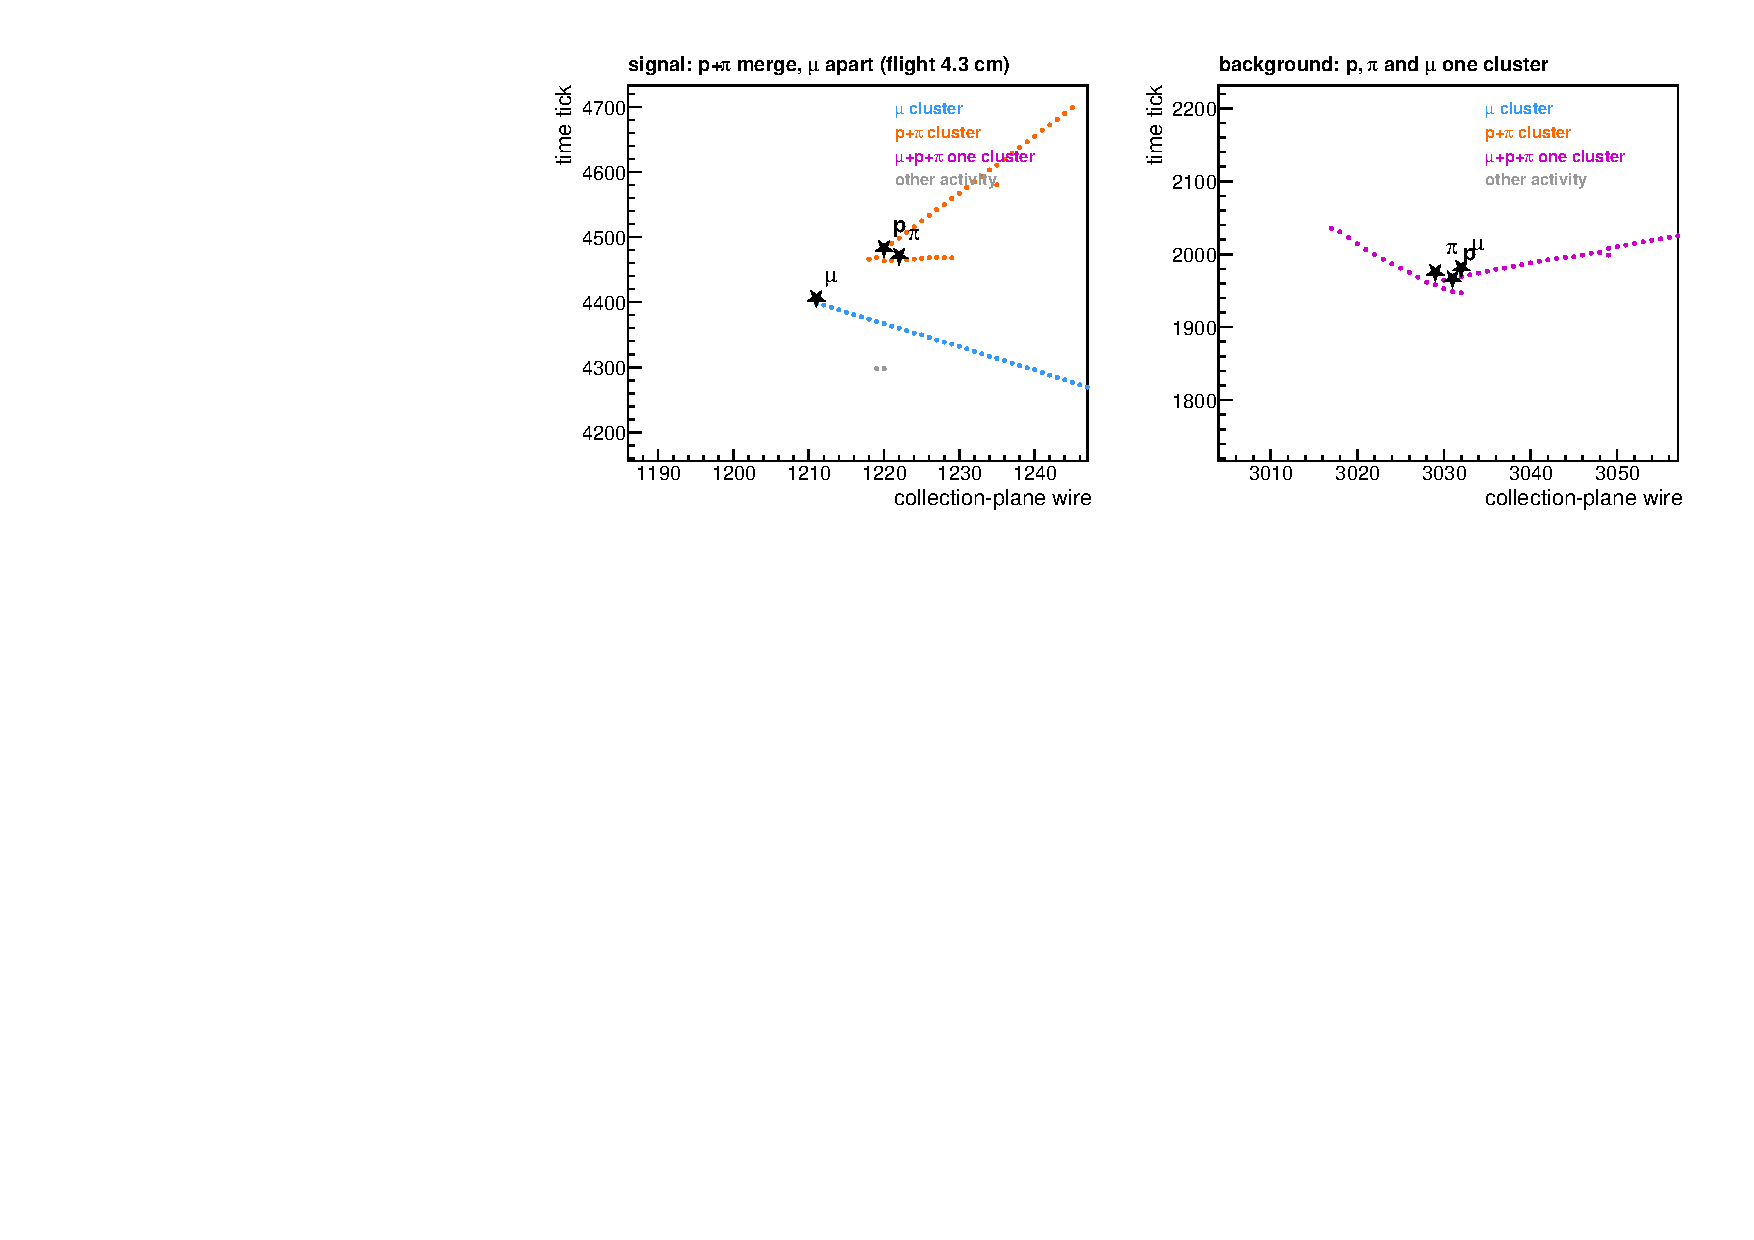
\includegraphics[width=\textwidth]{island_display.pdf}
\caption{The island test on the collection plane. Left: a GENIE signal event with
$4.3$~cm true \Lam\ flight; the proton and pion seeds share a cluster (orange) and
the muon has its own (blue). Right: a background event at the same stage, whose
proton, pion and muon seeds land in one cluster.}
\label{fig:island}
\end{figure}

\paragraph{Connectivity is tuned.} The original $3$ wires $\times$ $40$ ticks bridged
the decay V to the muon whenever the \Lam\ flew less than $\sim3$~cm, because 40
ticks is $2.2$~cm of drift. $2\times20$ lifts the signal pass rate:

\begin{center}
\begin{tabular}{lrrrr}
\toprule
true flight & 1--2 cm & 2--3 cm & 3--5 cm & 5--10 cm \\
\midrule
$3\times40$ (old) & $19\%$ & $45\%$ & $70\%$ & $86\%$ \\
$2\times20$ (now) & $43\%$ & $80\%$ & $85\%$ & $91\%$ \\
\bottomrule
\end{tabular}
\end{center}

\noindent On one plane the figure of merit is flat in the connectivity; the gain is
from requiring two planes ($6.8\times$ background rejection against $3.7\times$).
The tuning used the Run~3 overlay list; re-scanned with the choice made on Run~3 and
the score taken on the independent extension, the extension's figure of merit is a
plateau ($0.425$--$0.438$) and $2\times20$ is $0.004$ from its top. The two-plane pass
rate is the same for both generators: $50.5\%$ of NuWro, $50\%$ of GENIE.

\subsection{Operating point}

\Lam\ mass within $\pm20$~MeV, decay length $>0.5$~cm, $\cos\alpha>0.95$, photon start
$>2$~cm from the vertex, island test passed on $\geq2$ planes. GENIE signal from the
hyperon sample, background from the full hypana overlay:

\begin{table}[h]\centering
\caption{\Lam-style cut flow. Errors are MC statistics.}
\label{tab:lscutflow}
\begin{tabular}{lrrrr}
\toprule
stage & raw signal & raw background & $S$ (GENIE) & $B$ \\
\midrule
AllEvents                 & 15043 & 1840942 & 290.1 & 301031 \\
SliceID                   &  7801 &  776242 & 150.4 & 126931 \\
MuonCandidate             &  3043 &  123000 &  58.7 &  20113 \\
PairCandidate             &   921 &   51238 &  17.8 &   8378 \\
\Lam\ mass $\pm20$~MeV    &   504 &   16391 &  9.72 &   2680 \\
pointing ($\cos\alpha$, decay length) & 144 & 706 & 2.78 & 115.4 \\
photon gap $>2$~cm        &   139 &     549 &  2.68 &   89.8 \\
\textbf{island, $\geq2$ planes} & \textbf{69} & \textbf{23} & $\mathbf{1.33\pm0.16}$ & $\mathbf{3.76\pm0.78}$ \\
\bottomrule
\end{tabular}
\end{table}

\noindent Absolute efficiency $0.46\%$ (GENIE) and $0.42\%$ (NuWro), purity $26\%$
before EXT. $98.6\%$ of the surviving signal has true \Lam\ flight $>2$~cm, against
$43\%$ in the BDT chain. With the NuWro signal the same point gives
$S = 0.142\pm0.009$ (245 raw). NuWro's own non-signal events, \Szero\ that FSI turned
into something else (mostly \Lam), add $0.021\pm0.003$ background events (37 raw).
With EXT (Sec.~\ref{sec:ext}) $B = 4.40$ and the purity is $23\%$ (GENIE hyperon
sample) or $19\%$ (plain-overlay normalisation).

\begin{figure}[h]\centering
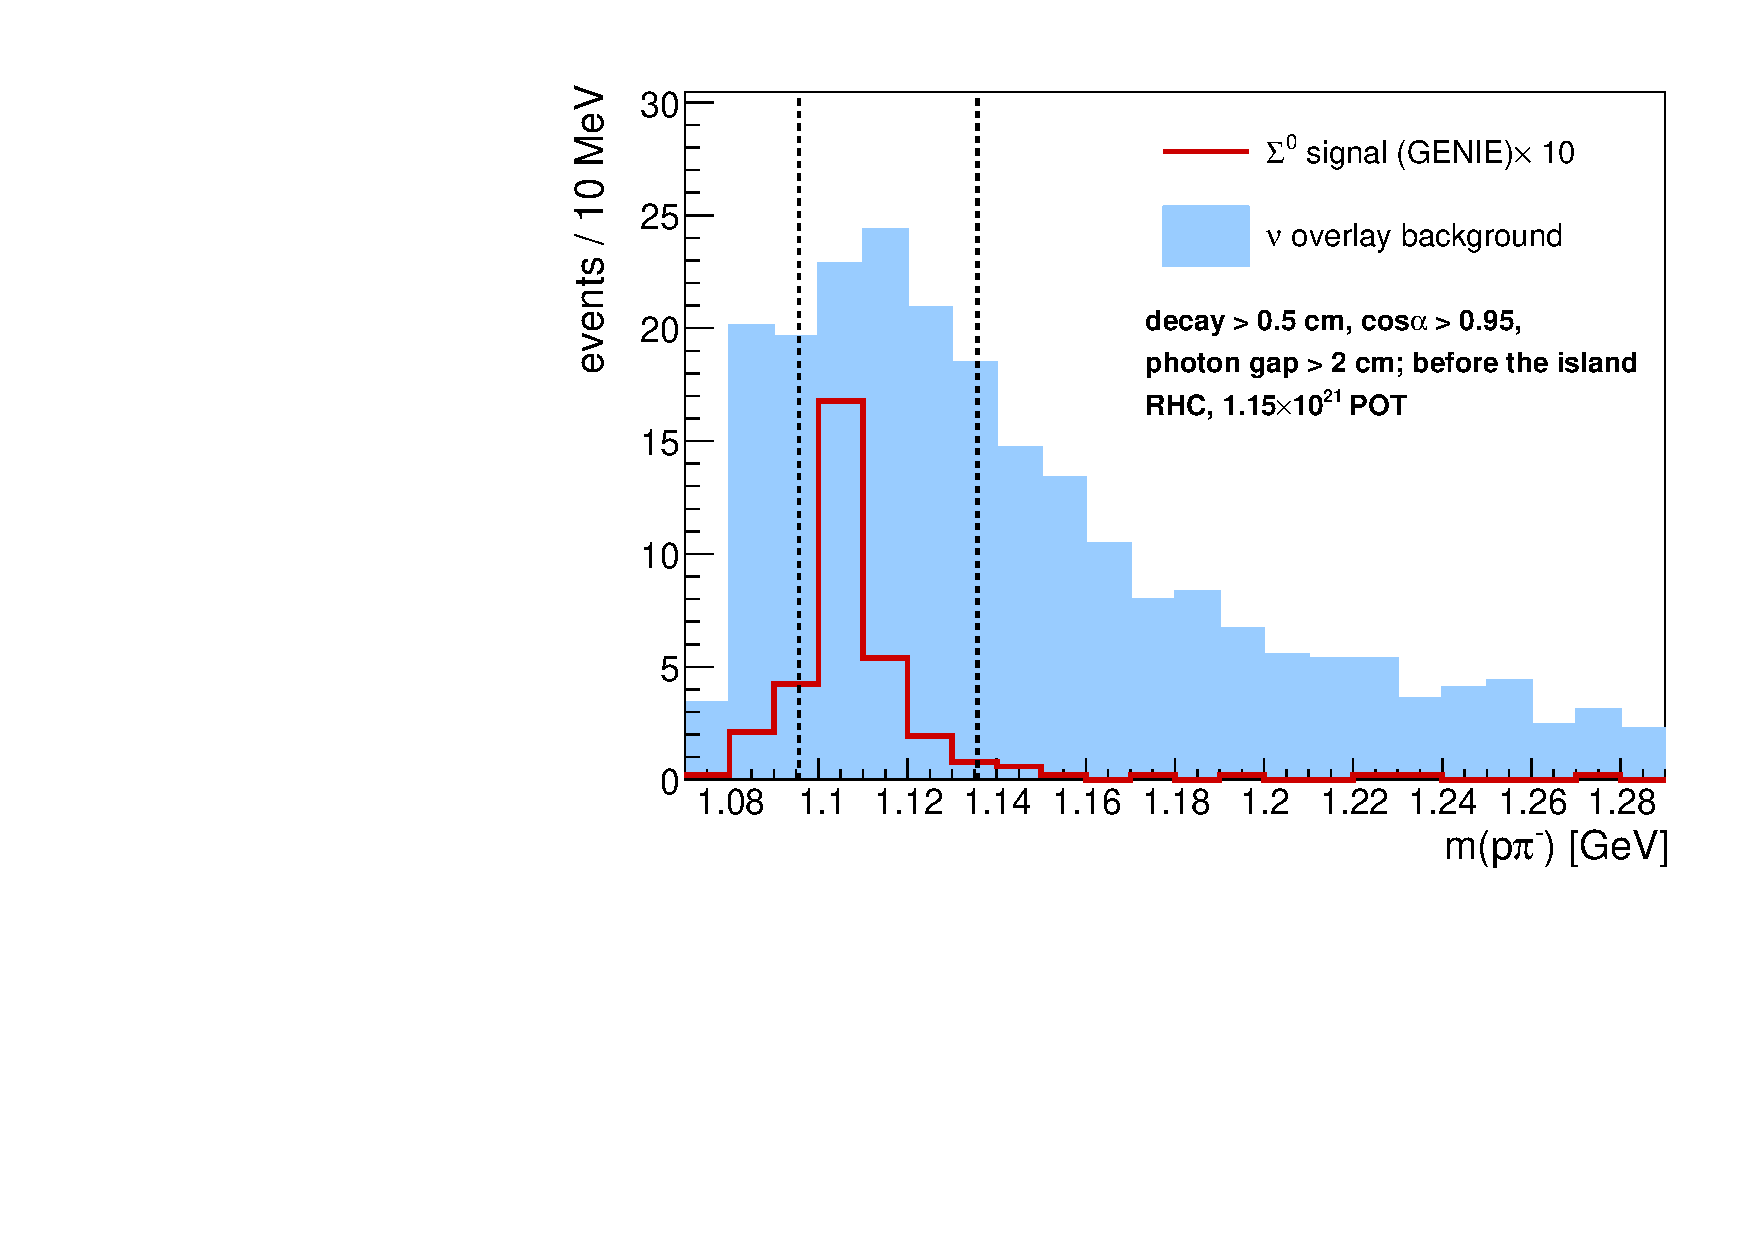
\includegraphics[width=0.62\textwidth]{lambda_mass.pdf}
\caption{$p\pi^-$ mass after the pointing cut and the photon gap, before the mass
window (dashed) and the island test. The signal peak sits slightly low because the
pion momentum is taken from range under the muon hypothesis, which is $20\%$ low for
a pion but gives a narrower peak than any correction. The background is largely
genuine $p\pi$ from $\Delta$ decay, whose mass sits just above threshold.}
\label{fig:lmass}
\end{figure}

\paragraph{Out-of-sample checks.} Without the gap, the original Run~3 list gives
$B = 4.15\pm1.31$ (10 raw) and the independent extension $7.6\pm1.4$ (28 raw); every
stage up to the pointing cut agrees per POT between the two to $1$--$4\%$, so the
low Run~3 value is a fluctuation of the sample the island test was tuned on. The
photon gap was fixed in September on the Run~3 list; on the extension it halves the
background ($7.56\to4.05$) at $96\%$ signal efficiency. Odd/even cross-validation
chooses the same configuration in both folds.

\paragraph{The photon and Michel handles.} $18.7\%$ of background ``photons'' start
within $2$~cm of the vertex against $3.5\%$ of signal; at two planes 11 of the 15
events the gap removes are hadrons reconstructed as a shower at the vertex. The
threshold sits on a plateau from 1 to 8~cm. A Michel tag (a contained muon with
another PFP within $5$~cm of its end) exploits that the background muon is a
wrong-sign $\mu^-$ $78\%$ of the time and is captured $75\%$ of the time in argon. It
removes $87\%$ true $\mu^-$, but costs $22\%$ of signal and lowers the figure of merit
on top of the gap, so it is off.

\paragraph{Sidebands} (one-plane point, for statistics):

\begin{center}
\begin{tabular}{lrrrr}
\toprule
region & $S$ & $B$ & raw $B$ & $S/B$ \\
\midrule
signal region (blind)                    & 1.89 & 14.9 &  91 & $12.7\%$ \\
mass sideband, $+40$ to $+200$~MeV        & 0.02 & 10.5 &  64 & $0.2\%$ \\
$\alpha$ sideband, $0<\cos\alpha<0.8$    & 0.50 & 58.2 & 356 & $0.9\%$ \\
island-fail region                       & 0.79 & 74.9 & 458 & $1.1\%$ \\
\bottomrule
\end{tabular}
\end{center}

\noindent All three are RES/DIS-dominated, like the signal region. The mass sideband
exists only above the peak, because $m(p\pi)$ has a kinematic floor at $1.078$~GeV.

% =============================================================================
\section{Beam-off background in the \Lam-style chain}
\label{sec:ext}
% =============================================================================

The run3b \texttt{ext\_unbiased} files were taken through reco2 and
HyperonProduction locally: all 3\,349 swizzled files, $16\,570$ NuMI-EXT-triggered
events, every one of which reached the hypana ntuple. An unbiased event is one sampled
gate, so the sample holds $162\,912$ gates and each event stands for $150.25$ data
events; it has $0.67\%$ of the data's cosmic statistics.

That is too little to follow EXT to the operating point: none of the 76
MuonCandidate events reaches the pointing cut, and zero means $<346$ events at
$90\%$~CL. \texttt{ExtFactor.C} therefore factorises: EXT at MuonCandidate from the
hypana EXT, times the pass fraction to the operating point of the overlay's own
cosmic-dominated candidates (more than half of the selected slice's hits unmatched to
MC, i.e.\ overlaid cosmic data: 4\,220 of the 123\,000 cached events).

\begin{center}
\resizebox{\textwidth}{!}{%
\begin{tabular}{lrrrrr}
\toprule
step (cumulative) & EXT raw & EXT $P$ & MC cosmic raw & MC cosmic $P$ & MC all-bkg $P$ \\
\midrule
MuonCandidate & 76 ($11\,419\pm1\,310$) & -- & 4\,220 & -- & -- \\
pair & 8 & $0.105\pm0.035$ & 571 & $0.135\pm0.005$ & 0.42 \\
\Lam\ mass $\pm20$~MeV & 3 & $0.38\pm0.17$ & 165 & $0.289\pm0.019$ & 0.32 \\
pointing & 0 & 0 of 3 & 7 & $0.042\pm0.016$ & 0.043 \\
island $+$ gap & 0 & -- & 0 of 7 & -- & 0.0326 \\
\bottomrule
\end{tabular}}
\end{center}

\noindent \textbf{EXT at the operating point is $0.62\pm0.27$ events.} The cosmic MC
is used as far as the pointing cut, the last step with at least five cosmic events.
For the island and gap steps the estimate takes the neutrino-background rate
($3.3\%$); the cosmic MC alone gives 0 of 7 there, and without that assumption the
bound is EXT~$<6.2$ at $90\%$~CL. This is the open part of the estimate, and its
direction is not known.

The real cosmic data test the factorisation wherever they still have events. 8 of 76
EXT candidates have a pair, which agrees with the cosmic MC ($0.135$, $P(\leq8)=0.29$)
and excludes the neutrino-background rate ($0.42$ would predict 32,
$P=1.8\times10^{-9}$). Taking EXT's own counts instead of the cosmic MC fractions up to
the pair step gives $0.48$, and up to the mass window $0.62$.

Hypana EXT at MuonCandidate is $1.7\times$ the PeLEE beam-off at the PeLEE
MuonCandidate, while the two chains' overlay agrees there ($20\,113$ against
$20\,348$). The excess is cosmic-specific and expected: hypana's
\texttt{topological\_score} is the highest NuScore of any slice, not the
flash-matched slice's, which raises a cosmic-only event's score far more than a
neutrino event's. The MC cosmics use the same definition, so the selection is
consistent within hypana.

% =============================================================================
\section{Expected sensitivity}
\label{sec:sensitivity}
% =============================================================================

\subsection{Method}
\texttt{Sensitivity.C} gives the expected 90\%~CL upper limit on $\mu$, the \Szero\ rate
in units of a generator's prediction ($\mu=1$ is the model), for both chains under
both generators. Each chain is a single-bin counting experiment,
$n\sim\mathrm{Pois}(\mu S e + b)$:
\begin{itemize}
  \item $b$ is lognormal with mean $B$ and fractional width
        $\sqrt{r_{\mathrm{MC}}^2+f^2}$, where $r_{\mathrm{MC}}$ is the MC statistics of
        $B$ (EXT and dirt included; a component with no raw events left is given one
        event of its own weight) and $f$ is the background systematic, which is scanned;
  \item $e$ is lognormal with mean 1 and fractional width $\sqrt{g^2+r_S^2}$, where
        $g=20\%$ is a placeholder for flux, efficiency and POT and $r_S$ the signal MC
        statistics;
  \item the limit is Bayesian, with a flat prior in $\mu\geq0$ and $b$, $e$
        marginalised. Hybrid CL$_s$ is $4\%$ tighter throughout, and both reproduce the
        PDG table exactly for a known background;
  \item the expected limit is the limit at the median $n$ of $\mathrm{Pois}(B)$, with
        the band from the $16\%$ and $84\%$ quantiles;
  \item $Z_A$ is the median discovery significance with an uncertain background
        (Cowan et al., arXiv:1007.1727).
\end{itemize}
$\muUL = n_{\mathrm{UL}}(B,\sigma_b)/S$, so the generator only rescales the limit and the
cut that minimises it does not depend on the signal normalisation.

\subsection{Results}

\begin{table}[h]\centering
\caption{Median expected 90\%~CL limit on $\mu$, $g=20\%$. ``Re-optimised'' scans the
BDT cut from 0.50 to 0.95 for each $f$ (cut in brackets); its GENIE value is the
NuWro value divided by the GENIE/NuWro ratio measured at 0.759.}
\label{tab:limits}
\small
\begin{tabular}{rlrlrlr}
\toprule
$f$ & \multicolumn{2}{c}{PeLEE, BDTG $>0.759$} & \multicolumn{2}{c}{PeLEE, re-optimised} & \multicolumn{2}{c}{\Lam-style} \\
 & NuWro [16--84\%] & GENIE & NuWro (cut) & GENIE & NuWro [16--84\%] & GENIE \\
\midrule
 0\% & 18.1 [12.8, 26.2] & 2.95 & 18.1 (0.750) & 2.91 & 36.9 [25.6, 51.9] & 5.33 \\
 5\% & 24.1 & 3.93 & 22.6 (0.850) & 3.65 & 37.0 & 5.34 \\
10\% & 35.7 & 5.84 & 27.1 (0.875) & 4.37 & 37.2 & 5.37 \\
15\% & 48.2 [41.4, 56.2] & 7.88 & 31.0 (0.890) & 5.00 & 37.6 [25.9, 52.7] & 5.43 \\
20\% & 60.3 & 9.85 & 34.0 (0.905) & 5.48 & 38.1 & 5.50 \\
30\% & 82.3 [74.4, 90.9] & 13.45 & 38.2 (0.925) & 6.16 & 39.3 [26.9, 54.8] & 5.68 \\
\bottomrule
\end{tabular}
\end{table}

\begin{figure}[h]\centering
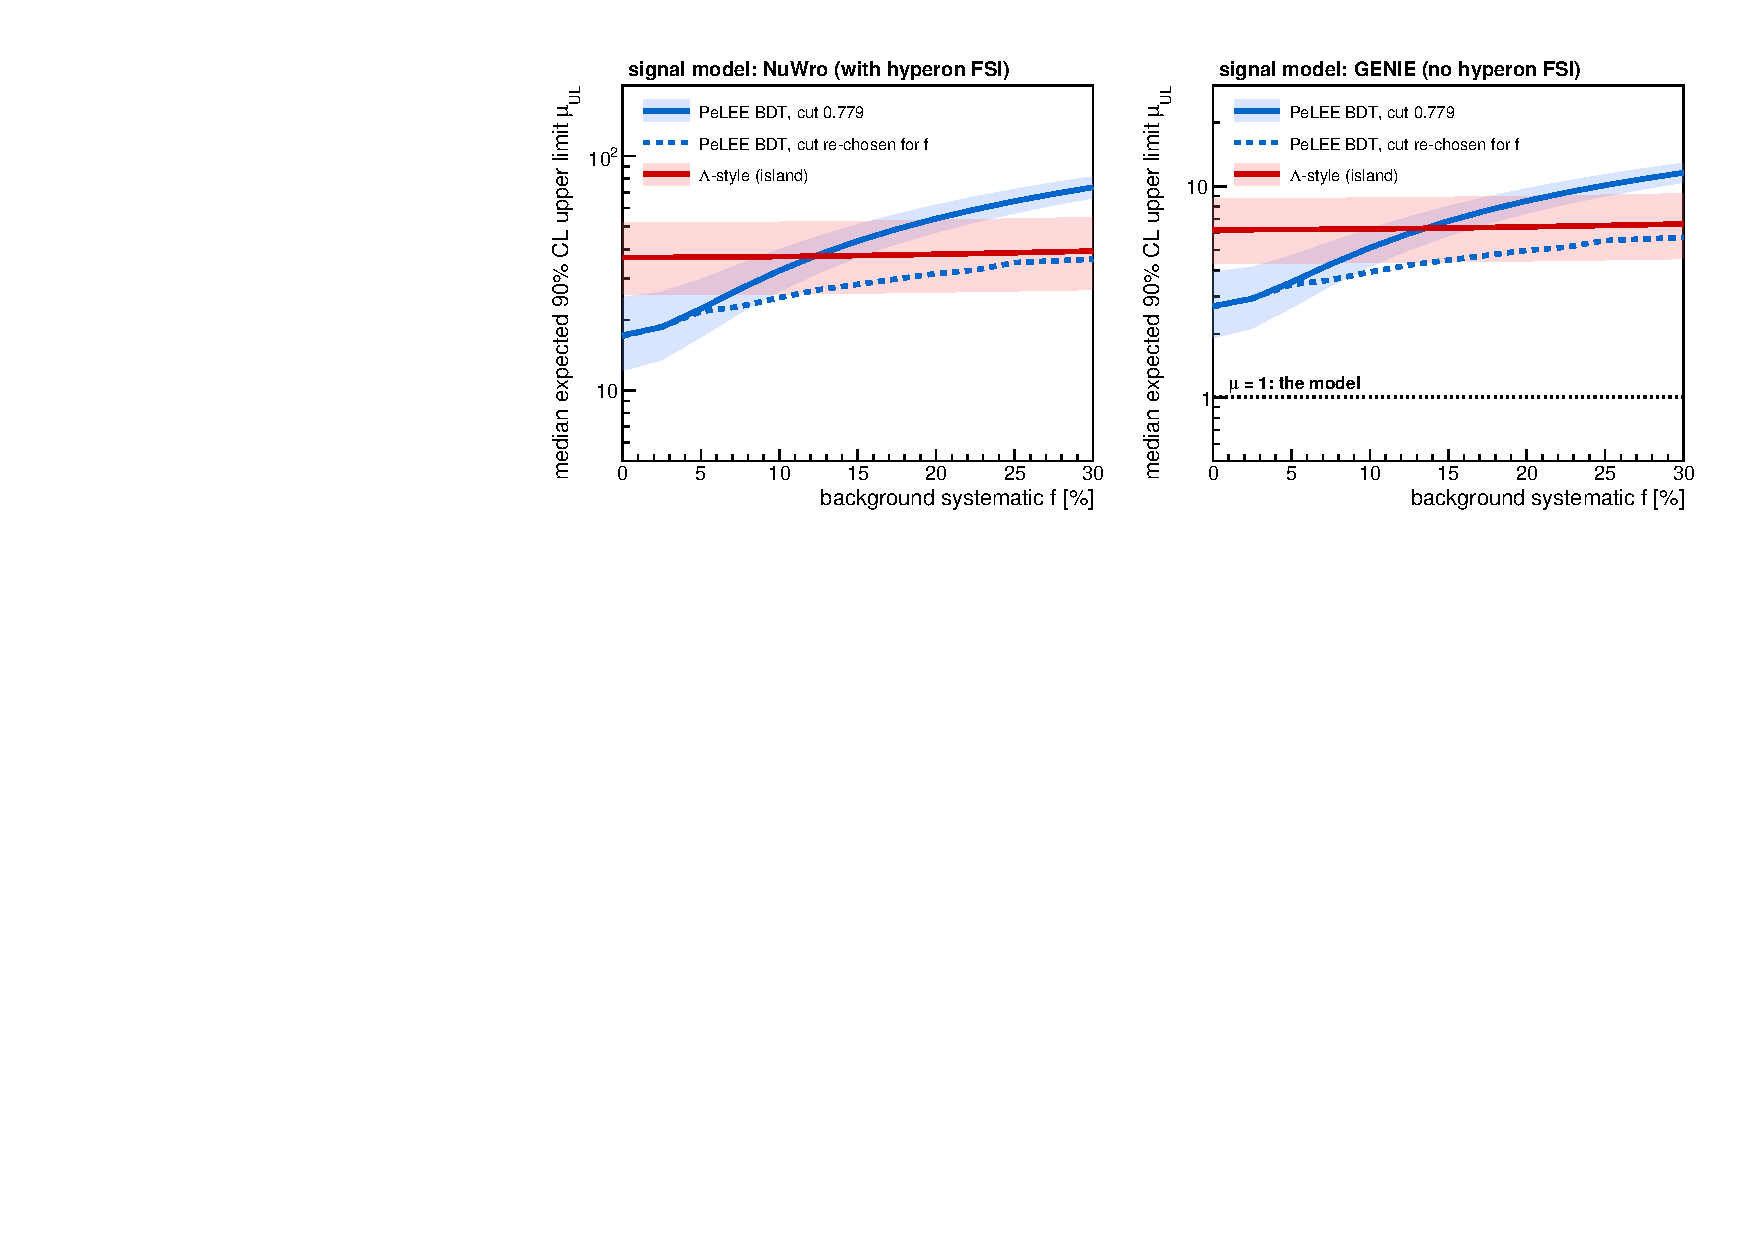
\includegraphics[width=\textwidth]{limit_vs_f.pdf}
\caption{Median expected 90\%~CL limit on $\mu$ against the background systematic,
under NuWro (left) and GENIE (right). Bands are the 16--84\% range; the dotted line on
the right is the GENIE prediction itself.}
\label{fig:limit}
\end{figure}

\begin{enumerate}
  \item \textbf{The result will be a limit.} The best median significance at the model
        rate is $0.63\sigma$ (GENIE, PeLEE, $f=0$) and $0.10\sigma$ under NuWro. The best
        expected limit, about $3\times$ GENIE and $18\times$ NuWro, is about 220 in-FV
        \Szero\ events in $1.15\times10^{21}$~POT, against 73 predicted by GENIE and 13
        by NuWro. In events the two models agree to $6\%$ (227 and 214 at $f=0$),
        because the efficiencies do (Sec.~\ref{sec:geniesig}).
  \item \textbf{The PeLEE chain gives the better limit below $f\approx20\%$.} With its
        cut set for the systematic it is $2.0\times$ better than the \Lam-style chain
        at $f=0$, $1.4\times$ at $10\%$ and $1.2\times$ at $15\%$ (NuWro; GENIE
        $1.8\times$, $1.2\times$, $1.1\times$). From 20 to 30\% the two are within
        $10\%$ and the model decides: NuWro keeps the PeLEE chain ahead (38.2 against
        39.3 at $30\%$), GENIE puts the \Lam-style chain ahead (5.7 against 6.2), because
        the two chains' GENIE/NuWro ratios differ (6.2 and 7.1). The \Lam-style chain's
        purity is real, but its signal yield is $15\times$ lower, and at $B\approx4.4$ its
        limit is set by Poisson counting: removing all background uncertainty moves it
        by $3\%$. This reverses the conclusion of the earlier comparison by
        $S/\sqrt{S+B+(fB)^2}$, which set the \Lam-style chain against the older hypana
        BDT, used the GENIE hyperon-sample normalisation, and kept each cut where it had
        been chosen at $f=0$.
  \item \textbf{The background systematic drives the PeLEE result.} From $f=0$ to
        $15\%$ its limit grows $1.7\times$ with the cut re-optimised and $2.7\times$ at
        0.759. At $f=10\%$ moving the cut from 0.759 to 0.875 improves the limit by
        $25\%$. The counting figure of merit agrees with the limit up to $f=10\%$; beyond
        it, it picks cuts whose $B$ rests on a few raw events (0.940, $B=6.3$) and is
        $1.7\times$ worse.
  \item \textbf{Nothing missing from the \Lam-style chain changes its limit by much.}
        At $f=15\%$ (NuWro, Poisson median): without the EXT estimate $39.8$ against
        $37.6$; with dirt at its bound ($+0.33\pm0.33$, the PeLEE dirt/overlay ratio at
        MuonCandidate) $43.5$; with $g=0$ $34.4$; with $B$ known exactly $36.5$. The
        median $n$ is an integer, so a small change in $B$ moves the median limit in
        steps, either way. Hypana data and dirt would give the \Lam-style chain an
        independent result with different systematics, not a better limit.
\end{enumerate}

% =============================================================================
\section{A global hypothesis fit}
\label{sec:hypfit}
% =============================================================================

\emph{Status: not built.} Its central idea, assigning the proton and pion jointly
instead of one after the other, is realised by the pair scoring of \texttt{PidAssign.h}
and of the \Lam-style chain. The full four-role fit below remains a possible
improvement; the reasoning and the measured ingredients are kept.

\subsection{Motivation}

The sequential selection identifies the muon, then the proton, then the pion, each
conditioned only on what has already been taken, and never uses the fact that
$p\pi^-$ must form a \Lam\ and $\Lam\gamma$ a \Szero. The per-role PID templates show
why this fails specifically on the pion: the muon, proton and photon each have a
distinctive signature, while the $\pi^-$ lies between the other three on every variable
measured. The proposed fit relaxes the candidate pool (every PFP eligible for every
role, recovering the $11.6\%$ of $\pi^-$ called showers), enumerates the $P(N,4)$
assignments, scores each with a combined $-2\ln L$ from the two mass constraints, the
per-role PID templates, muon-at-vertex, the $p$--$\pi$ DCA, a length-ordering prior and
a soft-photon prior, and admits partial hypotheses for the $29.1\%$ of signal with three
PFPs. Perfect assignment given what is found is worth a factor $1.54$ on $N\geq4$
events.

\subsection{Measured ingredients}

Recorded in \texttt{HypFitParams.h} (1323 signal events): \Lam\ mass constraint
centred at $1.1234$~GeV with $\sigma=27.2$~MeV and \Szero\ at $1.1812$~GeV with
$45.4$~MeV, from correctly assigned candidates. The \Lam\ width predates the
proton-momentum fix of Sec.~\ref{sec:recostudy}, which narrows it to $7.8$~MeV; it
must be remeasured before use. The $\chi^2$ must be centred on the measured means,
not the PDG masses. The $p$--$\pi$ DCA has median $0.35$~cm ($16$--$84\%$:
$0.08$--$1.36$~cm); the muon is the longest track $92.1\%$ of the time; and $98.9\%$
of PFPs carry both a track and a shower fit, so the relaxed pool needs no
re-reconstruction.

\begin{table}[h]\centering\small
\begin{tabular}{lrrrr}
\toprule
variable & $\mu^+$ & $p$ & $\pi^-$ & $\gamma$ \\
\midrule
\texttt{trk\_shr\_score}    & $1.00$  & $0.90$  & $0.80$  & $\mathbf{0.11}$ \\
\texttt{trk\_llrpid}        & $\mathbf{0.96}$ & $-0.29$ & $0.14$ & $0.56$ \\
\texttt{trk\_pid\_chipr}    & $180$   & $\mathbf{16.4}$ & $96$ & $192$ \\
\texttt{three\_plane\_dedx} & $2.47$  & $\mathbf{10.3}$ & $7.52$ & $3.30$ \\
\texttt{rms\_deflection}    & $0.01$  & $0.01$  & $0.01$  & $\mathbf{0.08}$ \\
\texttt{moliere\_avg}       & $1.78$  & $6.18$  & $8.95$  & $\mathbf{13.3}$ \\
\texttt{trk\_length}        & $\mathbf{139}$ & $12.8$ & $10.8$ & $14.2$ \\
\bottomrule
\end{tabular}
\caption{Per-role PID templates, medians on truth-matched PFPs. The $\pi^-$ has no
distinctive signature.}
\label{tab:templates}
\end{table}

\paragraph{The mass-sculpting risk.} Choosing the combination that best fits $m_\Lam$
sculpts a \Lam-like peak out of combinatorics in background. If the fit is built, the
masses are used for assignment only and kept out of the BDT, and the machinery is run on
background alone to check for an induced peak.

% =============================================================================
\section{Fake data by Poisson throw}
\label{sec:fakedata}
% =============================================================================

The current ``data'' sample of the PeLEE chain is the NuWro signal file itself, scaled
by POT. That is not a closure test: it contains no background and no fluctuation.

The fix is the Poisson-throw scheme of the CC$1\mu1\pi$ analysis
(\texttt{macros/throw\_perrun\_*.C}): for each MC event with central-value weight
$w_{\mathrm{cv}}$ and POT scale $\alpha$, draw $n \sim \mathrm{Poisson}(w_{\mathrm{cv}}
\alpha)$ and write the event $n$ times with unit weight, across all samples. EXT, a data
sample, enters at its scale directly. A \texttt{throw\_sigma0.C} modelled on
\texttt{throw\_perrun\_w.C}, one seed per sample, would provide it.

A throw from the same MC is a \emph{statistical} closure test, not a model test. A
model test needs a signal from a different generator in PeLEE format, and one now
exists: the overlay's own GENIE \Szero\ events, which the selection counts separately
(Sec.~\ref{sec:geniesig}). They are 187 raw events at the operating point, enough to
inject a GENIE signal into a throw of the NuWro-based prediction.

% =============================================================================
\section{Framework port}
\label{sec:port}
% =============================================================================

The selection was to be ported into \texttt{xsec\_analyzer} as a
\texttt{SelectionBase} subclass to inherit its systematic machinery (flux multisims,
GENIE multisims and unisims, detector variations, reinteraction), at a single analysis
bin. \textbf{Status, 2026-10-19: not started.} No \texttt{Sigma0} class exists, there
is no factory registration, and nine branches the selection uses are unbound in
\texttt{Branches.hh} (details in \texttt{SIGMA0\_FRAMEWORK\_PLAN.md}).

The port is no longer on the critical path. The PeLEE ntuples carry the multisim
weights themselves (\texttt{weightsGenie}, \texttt{weightsPPFX}, \texttt{weightsFlux},
\texttt{weightsReint}), the detector variations already run through the standalone
selection (Sec.~\ref{sec:detvar}), and \texttt{Sensitivity.C} provides the limit
machinery the framework lacks. A single-bin background covariance can be built in
\texttt{SigmaSelection.C} directly.

% =============================================================================
\section{Exposure: combined FHC$+$RHC later}
\label{sec:exposure}
% =============================================================================

The signal is $\numubar$ charged-current, so RHC is the sensitive mode. FHC carries a
substantial wrong-sign $\numubar$ component ($34.0\%$ of the FHC flux, against $53.3\%$
in RHC) and an exposure of $8.857\times10^{20}$~POT, so folding it in adds real signal.
The CC$1\mu1\pi$ analysis has the machinery: per-run POT scaling, a combined
\texttt{file\_properties} and combined flux normalisation. It needs FHC overlay
through the same selection, an FHC signal sample (or a justified reuse of the RHC
one), FHC dirt and FHC EXT. At the purity of the PeLEE chain the background grows with
the signal, so this is worth doing only once the systematics of Sec.~\ref{sec:plan}
are in hand.

% =============================================================================
\section{Work plan}
\label{sec:plan}
% =============================================================================

\begin{enumerate}
  \item \textbf{Background systematics for the PeLEE chain (priority).} The expected
        limit grows $1.7\times$ from $f=0$ to $15\%$, so this sets the result. Flux
        (\texttt{weightsPPFX}), cross section (\texttt{weightsGenie}) and reinteraction
        (\texttt{weightsReint}) multisims at the single bin, with the detector variations
        ($\lesssim7\%$, Sec.~\ref{sec:detvar}). Then a constraint from data: a fit of the
        BDT-score region where the signal is negligible, extrapolated to the signal
        region, which leaves only the shape uncertainty in $f$. The $\pi^0$
        normalisation is the obvious target (Sec.~\ref{sec:glee}).
  \item \textbf{Choose the BDT cut from that budget} with the \texttt{Sensitivity.C}
        scan (0.875 at $f=10\%$, 0.890 at $15\%$), and re-measure the detector
        variations there: the CV keeps fewer raw events at tighter cuts.
  \item \textbf{Signal-model systematic.} Hyperon FSI is a factor $\sim4$ between the
        generators, and the GENIE samples disagree among themselves by
        $1.3$--$1.6\times$. The limit is quoted under both models; the residual GENIE
        normalisation has to be understood before either number is final.
  \item \textbf{Closure and fake data.} \texttt{throw\_sigma0.C}, all samples, with the
        GENIE overlay signal as an injected alternative model (Sec.~\ref{sec:fakedata}).
  \item \textbf{Unblinding and the observed limit.} RHC beam-on data exist in PeLEE
        format (\texttt{custom\_pelee\_ntuples}). \texttt{Sensitivity.C} gives the
        observed limit once $n$ is known; the absolute cross-section limit needs the
        integrated $\numubar$ flux and the argon target count in the FV.
  \item \textbf{\Lam-style chain as a cross-check.} Data and dirt through reco2 and
        HyperonProduction, as was done for EXT, would make it an independent
        measurement with different systematics. It does not improve the limit
        (Sec.~\ref{sec:sensitivity}), so it comes after the items above. The EXT
        factorisation of its island step is the open part of its background.
  \item \textbf{Housekeeping.} \texttt{AblateBDT.C} and \texttt{TrainAllPFP.C}, the
        hypana BDTs, still train on $25\%$ of the events (TMVA's default split). The
        \texttt{Shower1MoliereAvg} histogram range is in radians while the variable is
        in degrees, so that control plot is empty at the BDT stage.
  \item \textbf{Combined exposure}, FHC$+$RHC (Sec.~\ref{sec:exposure}), and the
        framework port (Sec.~\ref{sec:port}) if it is still wanted.
\end{enumerate}

\end{document}
